\documentclass[border=2pt]{standalone}
\usepackage{tikz}
\usetikzlibrary{matrix}
\begin{document}
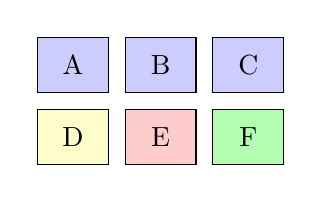
\begin{tikzpicture}
  \matrix (m) [matrix of nodes, row sep=2mm, column sep=2mm,
    nodes={draw,minimum width=9mm,minimum height=7mm},
    column 2/.style={nodes={fill=red!20}},
    every odd column/.style={nodes={fill=yellow!20}},
    row 1/.style={nodes={fill=blue!20}},
    row 2 column 3/.style={nodes={fill=green!30}}
  ] {
    A & B & C \\
    D & E & F \\
  };
\end{tikzpicture}
\end{document}
